\documentclass[a4paper,12pt]{article}
\usepackage[utf8]{inputenc}
\usepackage{hyperref}
\usepackage{graphicx}
\usepackage{float}
\graphicspath{ {images/} }

\begin{document}

\begin{titlepage}

\newcommand{\HRule}{\rule{\linewidth}{0.5mm}} % Defines a new command for the horizontal lines, change thickness here

\center % Center everything on the page
 
%----------------------------------------------------------------------------------------
%-	HEADING SECTIONS
%----------------------------------------------------------------------------------------

\textsc{\LARGE University of Pretoria}\\[1.5cm]
\textsc{\Large COS 301 - Software Engineering}\\[0.5cm]
\textsc{\large The Savage Ru's}\\[0.5cm]

%----------------------------------------------------------------------------------------
%-	TITLE SECTION
%----------------------------------------------------------------------------------------

\HRule \\[0.4cm]
{ \huge \bfseries Software Requirements Specification and Technology Neutral Process Design}\\[0.4cm] % Title of your document
\HRule \\[1.5cm]
 
%----------------------------------------------------------------------------------------
%-	AUTHOR SECTION
%----------------------------------------------------------------------------------------

\begin{minipage}{0.4\textwidth}
\begin{flushleft} \large
\emph{Author(s):}\\
Jodan \textsc{Alberts}\\ % Your name
Mark \textsc{Klingenberg}\\
Una \textsc{Rambani}\\
Ruan \textsc{Klinkert}\\
\end{flushleft}
\end{minipage}
~
\begin{minipage}{0.4\textwidth}
\begin{flushright} \large
\emph{Student number(s):} \\
14395283\\ % Student number
14020272\\
14004489\\
14022282\\

\end{flushright}
\end{minipage}\\[4cm]


%----------------------------------------------------------------------------------------
%-	DATE SECTION
%----------------------------------------------------------------------------------------

{\large \today}\\[3cm] % Date, change the \today to a set date if you want to be precise

 
%----------------------------------------------------------------------------------------

\vfill % Fill the rest of the page with whitespace

\end{titlepage}

\newpage

\tableofcontents

\newpage

\section{Introduction}

This is the software requirements specification for the vizARD Augmented Reality application being developed for EPI-USE Labs by The Savage Ru's.

\newpage
\section{Vision}
EPI-USE Labs (henceforth referred to as "the client") intends for the VizARD application to be used by a large variety of mobile device users across both Android and iOS platforms. VizARD helps to simplify the analysis of numerical data through visualization, in the form of automatically generated 3D graphs.

Fundamentally, the system will allow a user to take a picture of a table of numerical data which he/she may need to interpret. The application will then use OCR (Optical Character Recognition) to read the data from the picture. It will then decide on an appropriate graph for the type of data and generate a graph for the data. After the graph is generated, it will project a 3D model of the graph onto the image (or, ideally, onto a live stream of the paper) for the user to view.

Additionally, the system will allow users to send images (or screen captures) of generated graphs to other devices via popular social media channels.

Typically usage will be as follows:
\begin{itemize}
	\item The user (possibly a businessman) finds tabular data he/she would like to analyse more easily.
	\item The user opens the app.
	\item Once the app is open and loaded, the user takes a picture of the table he/she would like to analyse.
	\item The user receives a notification that the graph has been generated and the generated graph is displayed on the screen (mapped onto the paper).
	\item The user taps on the "Share" button and is presented with several options through which he/she can share the graph.
	\item An option is selected and an image of the graph is sent to the other user.
\end{itemize}

\newpage
\section{Background}

It is much simpler for us to recognize patterns and make quick analysis of data if it is presented to us in visual form. A simple example for the use of such an application would be a principal at a school who is presented with the Mathematics results of a particular grade for several quarters, such an application would make it very simple for him to quickly visualize the numeric data and see the trend.
\newline
\newline
The problem at hand is that there is a lot of information to go around and so little time to process. In a society that demands us to make decisions quickly, it would be wise to have a tool that aids the decision making process by making the information easier to digest and that is what vizARD intends to do.
\newline
\newline
Potential users could range from students, researchers, people in business, managers at stores and anyone else who would like to visualize data on the go.
		

\newpage
\section{Architecture Requirements}
In this section we discuss the software architecture requirements, including access and integration requirements, quality requirements and architectural constraints.

\subsection{Access Channel Requirements}
The system will function as an offline application. As such there will not be any outside system with direct access to the application. There are, however, access channels for user. Specifically users will gain access to the system via two mobile device operating system:
\begin{itemize}
	\item Android OS
	\item iOS
\end{itemize}

Furthermore any data that must be sent between the Operating System and the application will be done via the native APIs for each OS. On Android this will consist of the numerous Java APIs that is built into the system, and will likely be used to interact with the camera, file system, and (for sharing) the data connection. On iOS an Objective-C API suite will be used - in keeping with the native development philosophy of iOS.
\subsection{Quality Requirements}

\subsubsection{Performance}

\subsubsection{Reliability}

\subsubsection{Scalability}

\subsubsection{Usability} 

\subsubsection{Auditability}

\subsubsection{Security}

\subsection{Integration Requirements}
The VizARD app will integrate with Android OS, and iOS, and use the suite of Android APIs which accompany the OSes. Specifically, APIs will be used to integrate with the sharing functions in order to share to different social media platforms and messaging apps. Additionally the app will gain access to the file system and camera via the built-in APIs. Furthermore, Java APIs will be used to integrate between the various systems which make up VizARD's functionality. For instance between OpenCV and Tesseract for the OCR.

\subsection{Architecture Constraints}
\begin{itemize}
	\item Android
	\item iOS
\end{itemize}
Although no other specific constraints are specified, it is implied that the systems used must all be cross-platform to allow for the two different interfaces (Android and iOS). As such, the AR Engine, OCR Engine and 3D Library must be OS independent.

\subsection{Use case prioritization}
	\subsubsection{Critical}
		\begin{itemize}
			\item Taking a picture
			\item OCR (Optical Character Recognition)
			\item Automatic Graph Suggestion Algorithm
			\item Graph Generation
			\item Mapping Graph to Page
		\end{itemize}
	\subsubsection{Important}
		\begin{itemize}
			\item Live Augmented Reality Mapping
			\item Editing Graphs
			\item iOS Application
			\item Social Media Sharing
		\end{itemize}
	\subsubsection{Nice to Have}
		\begin{itemize}
			\item Opening Previous Graph
		\end{itemize}

\subsection{Use case/Services contracts}
	\begin{figure}[H]
		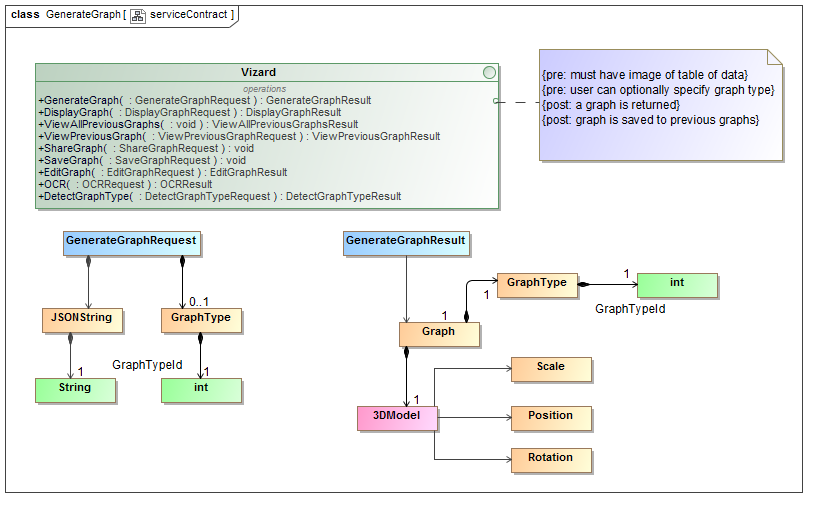
\includegraphics[width=\textwidth]{Images/class__GenerateGraph__serviceContract.png}  \\
		\caption{Services Contract : GenerateGraph}
	\end{figure}
	\begin{figure}[H]
		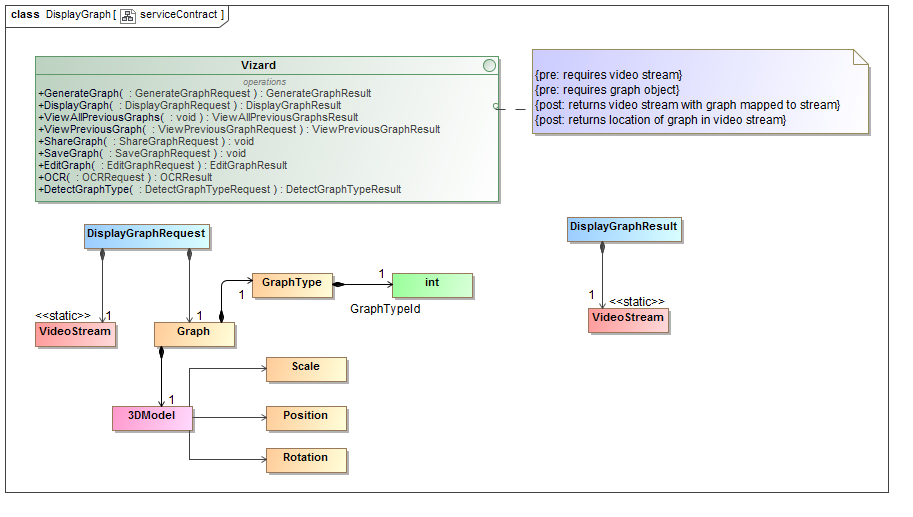
\includegraphics[width=\textwidth]{Images/class__DisplayGraph__serviceContract.png}  \\
		\caption{Services Contract : DisplayGraph}
	\end{figure}
	\begin{figure}[H]
		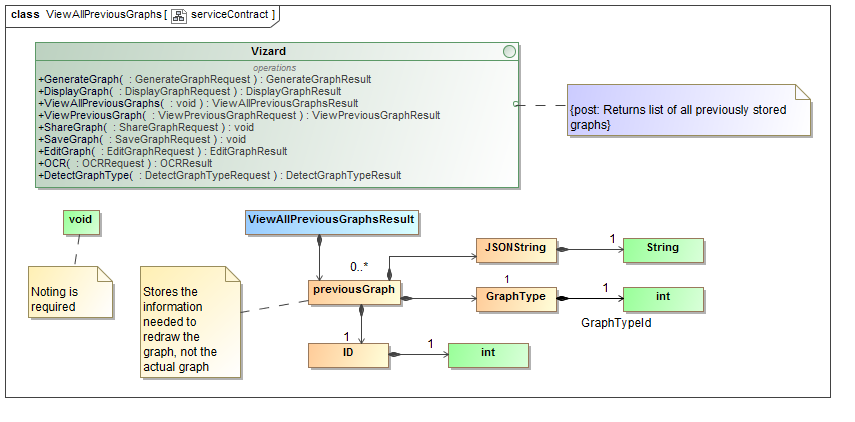
\includegraphics[width=\textwidth]{Images/class__ViewAllPreviousGraphs__serviceContract.png}  \\
		\caption{Services Contract : ViewAllPreviousGraphs}
	\end{figure}
	
	\begin{figure}[H]
		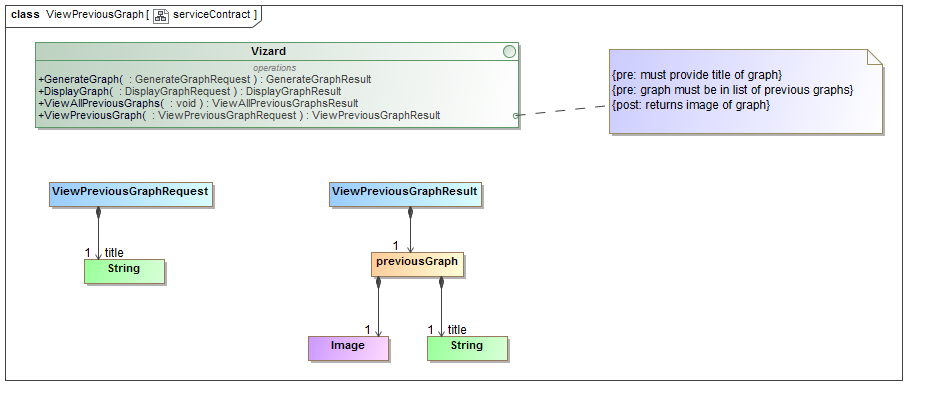
\includegraphics[width=\textwidth]{Images/class__ViewPreviousGraph__serviceContract.png}  \\
		\caption{Services Contract : ViewPreviousGraph}
	\end{figure}
	
	\begin{figure}[H]
		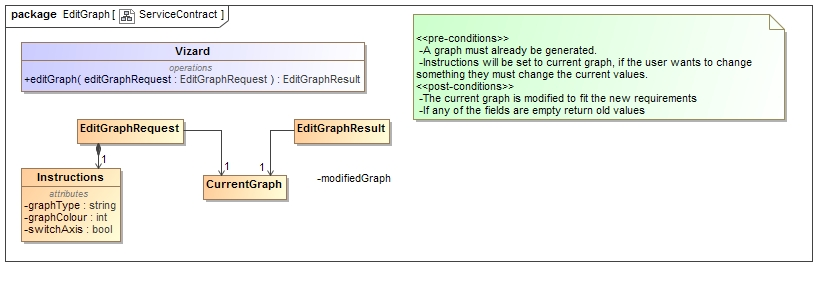
\includegraphics[width=\textwidth]{Images/class__EditGraph}  \\
		\caption{Services Contract : EditGraph}
	\end{figure}
	
	\begin{figure}[H]
		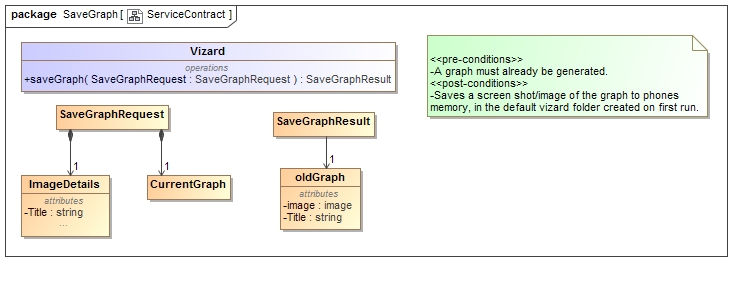
\includegraphics[width=\textwidth]{Images/class__SaveGraph}  \\
		\caption{Services Contract : SaveGraph}
	\end{figure}
	
	\begin{figure}[H]
		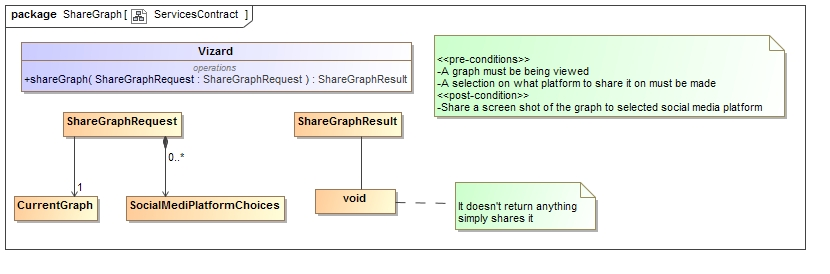
\includegraphics[width=\textwidth]{Images/class__ShareGraph}  \\
		\caption{Services Contract : ShareGraph}
	\end{figure}

\subsection{Required functionality}
	\begin{figure}[H]
		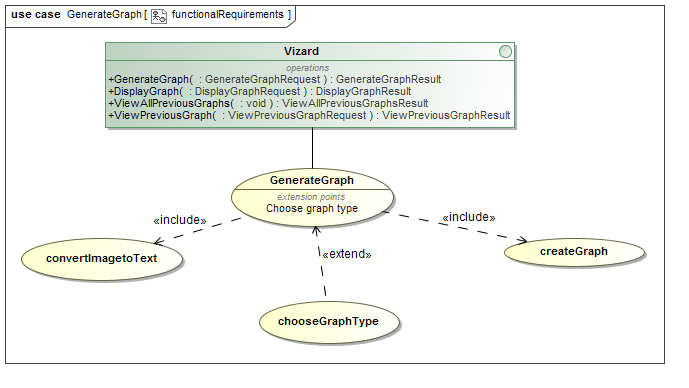
\includegraphics[width=\textwidth]{Images/uc__GenerateGraph__functionalRequirements.png}  \\
		\caption{Required functionality : GenerateGraph}
	\end{figure}
	\begin{figure}[H]
		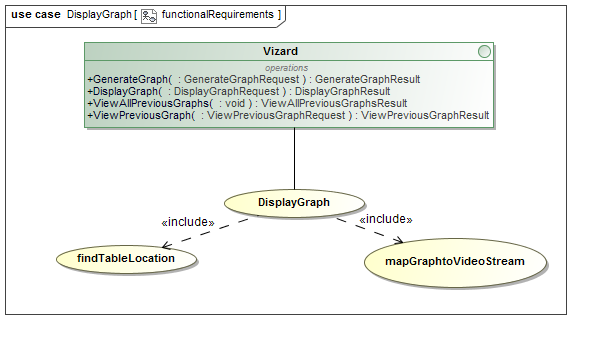
\includegraphics[width=\textwidth]{Images/uc__DisplayGraph__functionalRequirements.png}  \\
		\caption{Required functionality : DisplayGraph}
	\end{figure}
	\begin{figure}[H]
		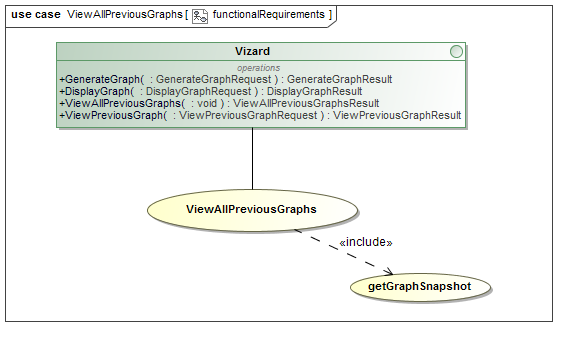
\includegraphics[width=\textwidth]{Images/uc__ViewAllPreviousGraphs__functionalRequirements.png}  \\
		\caption{Required functionality : ViewAllPreviousGraphs}
	\end{figure}
	\begin{figure}[H]
		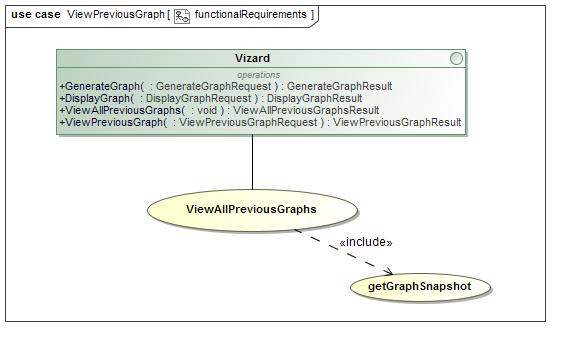
\includegraphics[width=\textwidth]{Images/uc__ViewPreviousGraph__functionalRequirements.png}  \\
		\caption{Required functionality : ViewPreviousGraph}
	\end{figure}	
	
	\begin{figure}[H]
		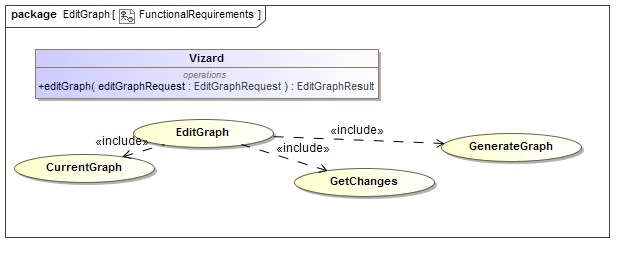
\includegraphics[width=\textwidth]{Images/uc__EditGraph}  \\
		\caption{Required functionality : EditGraph}
	\end{figure}
	
	\begin{figure}[H]
		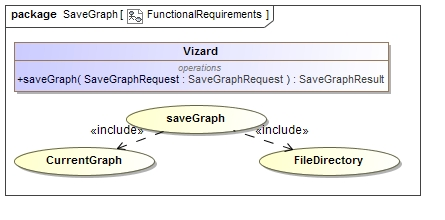
\includegraphics[width=\textwidth]{Images/uc__SaveGraph}  \\
		\caption{Required functionality : SaveGraph}
	\end{figure}
	
	\begin{figure}[H]
		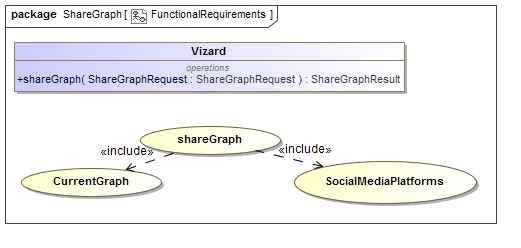
\includegraphics[width=\textwidth]{Images/uc__ShareGraph}  \\
		\caption{Required functionality : ShareGraph}
	\end{figure}

\subsection{Process specifications}
	\begin{figure}[H]
		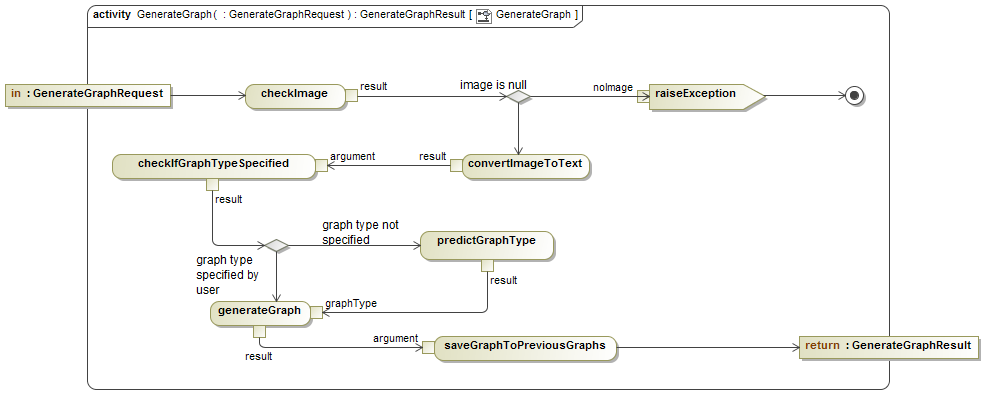
\includegraphics[width=\textwidth]{Images/act__GenerateGraph__GenerateGraph.png}  \\
		\caption{Process specifications : GenerateGraph}
	\end{figure}
	\begin{figure}[H]
		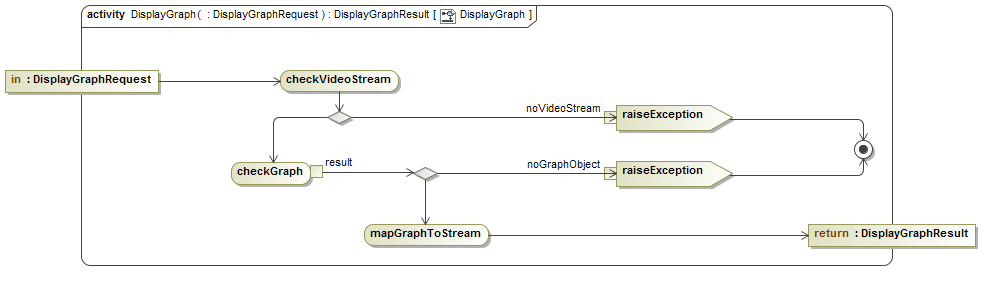
\includegraphics[width=\textwidth]{Images/act__DisplayGraph__DisplayGraph.png}  \\
		\caption{Process specifications : DisplayGraph}
	\end{figure}
	\begin{figure}[H]
		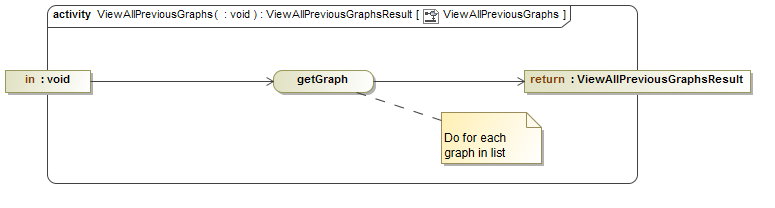
\includegraphics[width=\textwidth]{Images/act__ViewAllPreviousGraphs__ViewAllPreviousGraphs.png}  \\
		\caption{Process specifications : ViewAllPreviousGraphs}
	\end{figure}
	\begin{figure}[H]
		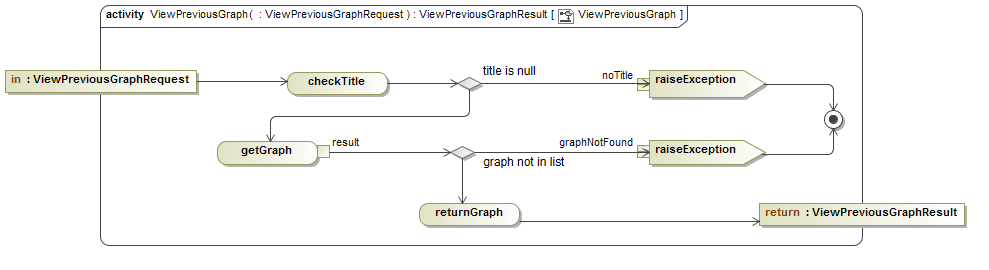
\includegraphics[width=\textwidth]{Images/act__ViewPreviousGraph__ViewPreviousGraph.png}  \\
		\caption{Process specifications : ViewPreviousGraph}
	\end{figure}
	
		\begin{figure}[H]
		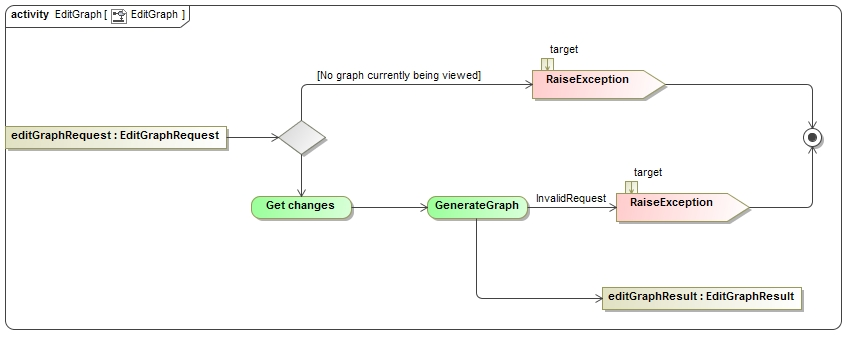
\includegraphics[width=\textwidth]{Images/act__EditGraph}  \\
		\caption{Process specifications : EditGraph}
	\end{figure}
	
	\begin{figure}[H]
		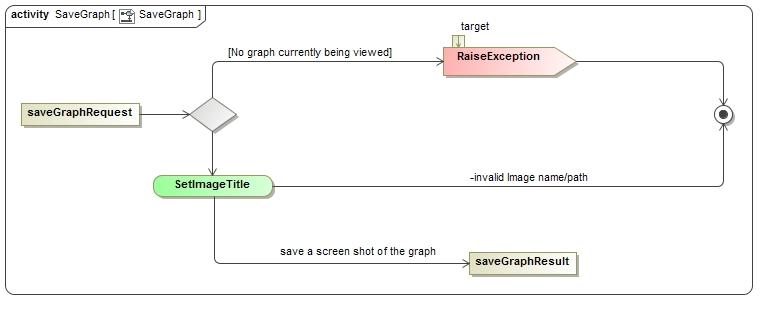
\includegraphics[width=\textwidth]{Images/act__SaveGraph}  \\
		\caption{Process specifications : SaveGraph}
	\end{figure}
	
	\begin{figure}[H]
		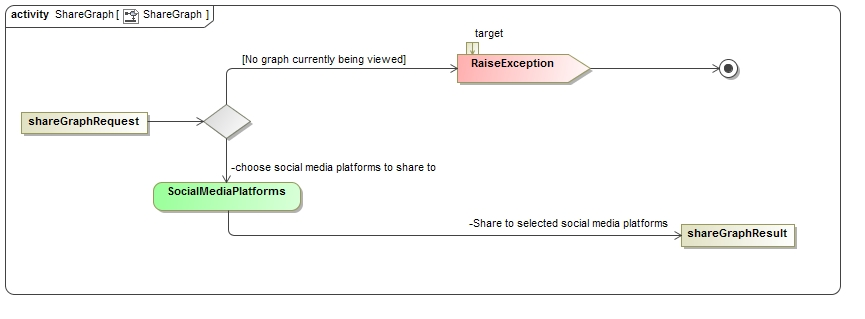
\includegraphics[width=\textwidth]{Images/act__ShareGraph}  \\
		\caption{Process specifications : ShareGraph}
	\end{figure}

\subsection{Domain Model}

\newpage
\section{Software Architecture}

\subsection{Architectural Patterns or Styles}

\subsection{Architectural Tactics or Strategies}

\subsection{Use of Reference Architectures and Frameworks}

\subsubsection{Web 2.0 Reference Architecture}

\subsection{Access and Integration Channels}

\subsection{Technologies}

\newpage
\section{Open Issues}


\end{document}
